\documentclass[a4paper, 25pt]{article}
\usepackage[utf8]{inputenc}
\usepackage[english,russian]{babel}
\usepackage{amsmath,amssymb,amsfonts,textcomp,latexsym,amsopn}
\usepackage{cite,enumerate,float,indentfirst}
\usepackage{graphicx,xcolor}
\usepackage{gnuplottex}
\begin{document}

\begin{flushright}
Кобзарев Алексей, Тескер Константин, Белозёров Михаил, Рыбаков Владислав.
\\
410 группа
\end{flushright}

\begin{center}
\bfseries ОТЧЕТ ПО ПРАКТИКУМУ НА ЭВМ
\end{center}

\section{Постановка задачи}

Была поставлена задача написания программы проводящей расчёт течения в каверне разностной схемой. 
Система уравнений, описывающая нестационарное движение баротропного газа в область $\Omega$ размерности два, выглядит следующим образом

\begin{equation}
% \frac{\partial p}{\partial t} + div(\rhou) = 0,\\
 \rho[\frac{\partial u}{\partial t} + (u, \bigtriangledown)u]  + \bigtriangledown p = Lu + \rho f, ~~
 p = p (\rho).
\end{equation}
где $L$ есть линейный симметричный положительно определенный оператор.

В данном случае рассматривалась схема описывающая поведение плотности и скорости газа в каверне.

\section{Гладкое решение}

Для проверки правильности формул и работы программы были проведены тесты на гладком решении. В качестве гладкого решения для плотности и скорости были выбраны следующие функции:

$$u1 = sin (2x) \cdot sin (2y) \cdot e^t$$
$$u2 = sin (2x) \cdot sin (2y) \cdot e^{-t}$$
$$\rho = (cos (2x) + 1.5) \cdot (sin (2y) + 1.5) \cdot e^t$$


Для проверки решения далее приведены значения норм разности решения и действительного значения для различных сеток, а также таблица времени работы программы.

\begin{center}
 $C$-норма ошибки для $g: \quad p_{\rho}=10.000, \mu = 0.010 $
\begin{tabular}{|p{0.6in}|p{0.7in}|p{0.7in}|p{0.7in}|p{0.7in}|} \hline
$\tau\setminus h$ & $0.05$ & 0.025& 0.0125 & 0.00625 \\ \hline
$0.01000$ & $5.748e-02$ &$1.321e-01$ &$1.555e-01$ &$1.607e-01$  \\ \hline
$0.00500$ & $5.561e-02$ &$1.292e-01$ &$1.544e-01$ &$1.577e-01$  \\ \hline
$0.00250$ & $5.467e-02$ &$1.282e-01$ &$1.539e-01$ &$1.543e-01$  \\ \hline
$0.00125$ & $5.420e-02$ &$1.267e-01$ &$1.507e-01$ &$1.541e-01$  \\ \hline
\end{tabular}\\[20pt]
\end{center}

\begin{center}
 $L_2$-норма ошибки для $g: \quad p_{\rho}=10.000, \mu = 0.010 $
\begin{tabular}{|p{0.6in}|p{0.7in}|p{0.7in}|p{0.7in}|p{0.7in}|} \hline
$\tau\setminus h$ & $0.05$ & 0.025& 0.0125 & 0.00625 \\ \hline
$0.01000$ & $2.898e-02$ &$3.514e-02$ &$3.661e-02$ &$3.636e-02$  \\ \hline
$0.00500$ & $2.783e-02$ &$3.490e-02$ &$3.655e-02$ &$3.632e-02$  \\ \hline
$0.00250$ & $2.729e-02$ &$3.481e-02$ &$3.639e-02$ &$3.632e-02$  \\ \hline
$0.00125$ & $2.703e-02$ &$3.477e-02$ &$3.633e-02$ &$3.632e-02$  \\ \hline
\end{tabular}\\[20pt]
\end{center}

\begin{center}
$C$-норма ошибки для $v1: \quad p_{\rho}=10.000, \mu = 0.010 $
\begin{tabular}{|p{0.6in}|p{0.7in}|p{0.7in}|p{0.7in}|p{0.7in}|} \hline
$\tau\setminus h$ & $0.05$ & 0.025& 0.0125 & 0.00625 \\ \hline
$0.01000$ & $3.384e-01$ &$2.154e-01$ &$2.259e-01$ &$4.563e-01$  \\ \hline
$0.00500$ & $3.199e-01$ &$2.115e-01$ &$2.233e-01$ &$4.503e-01$  \\ \hline
$0.00250$ & $3.181e-01$ &$2.106e-01$ &$2.231e-01$ &$4.496e-01$  \\ \hline
$0.00125$ & $3.092e-01$ &$2.096e-01$ &$2.223e-01$ &$4.487e-01$  \\ \hline
\end{tabular}\\[20pt]
\end{center}

\begin{center}
 $L_2$-норма ошибки для $v1: \quad p_{\rho}=10.000, \mu = 0.010 $
\begin{tabular}{|p{0.6in}|p{0.7in}|p{0.7in}|p{0.7in}|p{0.7in}|} \hline
$\tau\setminus h$ & $0.05$ & 0.025& 0.0125 & 0.00625 \\ \hline
$0.01000$ & $1.659e-01$ &$1.052e-01$ &$6.990e-02$ &$3.969e-02$  \\ \hline
$0.00500$ & $1.639e-01$ &$1.048e-01$ &$6.981e-02$ &$3.964e-02$  \\ \hline
$0.00250$ & $1.620e-01$ &$1.041e-01$ &$6.976e-02$ &$3.953e-02$  \\ \hline
$0.00125$ & $1.601e-01$ &$1.039e-01$ &$6.973e-02$ &$3.937e-02$  \\ \hline
\end{tabular}\\[20pt]
\end{center}

\begin{center}
 $C$-норма ошибки для $;v2: \quad p_{\rho}=10.000, \mu = 0.010 $
\begin{tabular}{|p{0.6in}|p{0.7in}|p{0.7in}|p{0.7in}|p{0.7in}|} \hline
$\tau\setminus h$ & $0.05$ & 0.025& 0.0125 & 0.00625 \\ \hline
$0.01000$ & $2.256e-01$ &$2.033e-01$ &$3.452e-01$ &$5.712e-01$  \\ \hline
$0.00500$ & $2.255e-01$ &$2.030e-01$ &$3.448e-01$ &$5.713e-01$  \\ \hline
$0.00250$ & $2.254e-01$ &$2.024e-01$ &$3.443e-01$ &$5.733e-01$  \\ \hline
$0.00125$ & $1.898e-01$ &$2.014e-01$ &$3.445e-01$ &$5.848e-01$  \\ \hline
\end{tabular}\\[20pt]
\end{center}

\begin{center}
$L_2$-норма ошибки для $v2: \quad p_{\rho}=10.000, \mu = 0.010  $
\begin{tabular}{|p{0.6in}|p{0.7in}|p{0.7in}|p{0.7in}|p{0.7in}|} \hline
$\tau\setminus h$ & $0.05$ & 0.025& 0.0125 & 0.00625 \\ \hline
$0.01000$ & $5.427e-02$ &$2.994e-02$ &$1.875e-02$ &$2.273e-02$  \\ \hline
$0.00500$ & $5.416e-02$ &$2.967e-02$ &$1.859e-02$ &$2.285e-02$  \\ \hline
$0.00250$ & $5.419e-02$ &$2.976e-02$ &$1.864e-02$ &$2.280e-02$  \\ \hline
$0.00125$ & $4.880e-02$ &$3.034e-02$ &$1.905e-02$ &$2.270e-02$  \\ \hline
\end{tabular}\\[20pt]
\end{center}

\begin{center}
Время, $p_{\rho}=10.000, \mu = 0.010  $
\begin{tabular}{|p{0.6in}|p{0.7in}|p{0.7in}|p{0.7in}|p{0.7in}|} \hline
$\tau\setminus h$ & $0.05$ & 0.025& 0.0125 & 0.00625 \\ \hline
$0.00010$ & $8.603e-03$ &$2.935e-02$ &$1.295e-01$ &$7.603e-01$  \\ \hline
$0.00005$ & $1.550e-02$ &$5.310e-02$ &$2.467e-01$ &$1.341e+00$  \\ \hline
$0.00003$ & $3.005e-02$ &$9.889e-02$ &$4.552e-01$ &$2.554e+00$  \\ \hline
$0.00001$ & $5.630e-02$ &$1.962e-01$ &$8.307e-01$ &$4.615e+00$  \\ \hline
\end{tabular}\\[20pt]
\end{center}


Результаты свидетельствуют о том, что программа реализована верно и имеет место сходимость решения к действительному значению плотности и скорости.
\newpage

\section {Численные эксперименты}

Были проведены численные эксперименты, моделирующие реальных условий.
Блыли реализованы четыре версии программы описываще различные по форме каверны.
Начальные условия были установлены следующие:\\
Белозёров Михаил
\begin {itemize}
\item Область $\Omega = \Omega_{02} \cup \Omega_{12} \cup \Omega_{22} \cup \Omega{11} \cup \Omega{21} \cup \Omega{10} \cup \Omega_{20}$
  \item $u_1|_{\Gamma_{02}^{x-}} = \omega$
  \item $\frac{{\partial}u_2}{{\partial}y}|_{\Gamma_{10}^{y-}\cup\Gamma_{20}^{y-}} = 0$
  \end   {itemize}
Кобзарев Алексей
\begin {itemize}
\item Область $\Omega = \Omega_{00} \cup \Omega_{10} \cup \Omega_{01} \cup \Omega{11} \\ \Gamma^{x+}_{00}$
  \item $u_2|_{\Gamma_{00}^{Y-}} = \omega$
  \item $\frac{{\partial}u_2}{{\partial}y}|_{\Gamma_{10}^{y-}} = 0$
\end   {itemize}
Рыбаков Владислав
\begin {itemize}
  \item Область $\Omega = \Omega_{00}\cup\Omega_{10}\cup\Omega_{11}\cup\Omega_{20}$
  \item $u_1|_{\Gamma_{00}^{x-}} = \omega$
  \item $\frac{{\partial}u_1}{{\partial}x}|_{\Gamma_{20}^{x+}} = 0$
  \item $\frac{{\partial}u_2}{{\partial}y}|_{\Gamma_{11}^{y+}} = 0$
\end   {itemize}
Тескер Константин
\begin {itemize}
  \item Область $\Omega = \Omega_{01}\cup\Omega_{10}\cup\Omega_{11}\cup\Omega_{12}$
  \item $u_1|_{\Gamma_{01}^{x-}} = \omega$
  \item $\frac{{\partial}u_2}{{\partial}y}|_{\Gamma_{12}^{y+}} = 0$
  \item $\frac{{\partial}u_2}{{\partial}y}|_{\Gamma_{10}^{y-}} = 0$
\end   {itemize}


Для выяснения корректности проведенных экспериментов была написана дополнительная программа, визуализирующая результаты проделанных экспериментов. Было замечено, что при увеличении временного парметра решение стабилизируется и результаты для каждой из задач выглядят следующим образом: \\
Белозёров Михаил:
\begin{figure}[h!]
\center{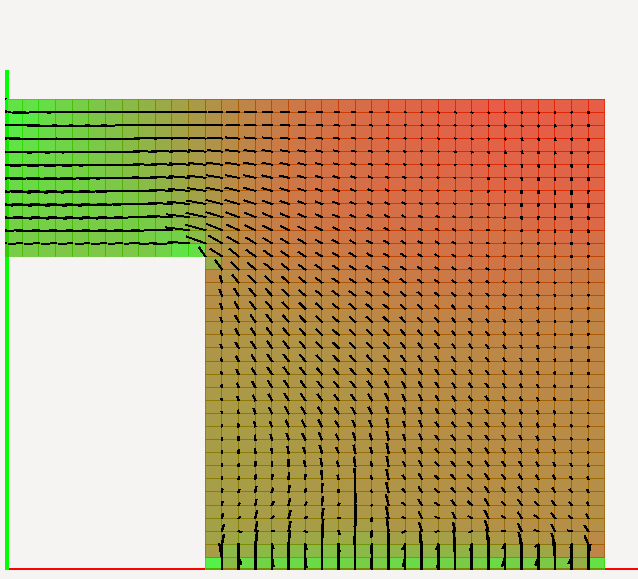
\includegraphics[width=0.7\linewidth]{screen_belozerov.jpg}}
\end{figure}
\\
\newpage
Кобзарев Алексей:
\begin{figure}[h!]
\center{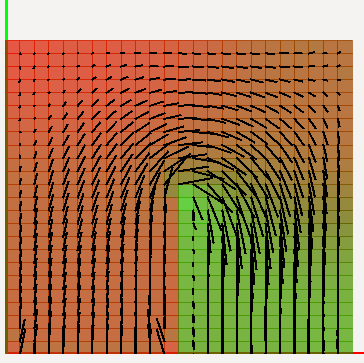
\includegraphics[width=0.7\linewidth]{screen_kobzarev.png}}
\end{figure}
\\
Рыбаков Владислав:
\begin{figure}[h!]
\center{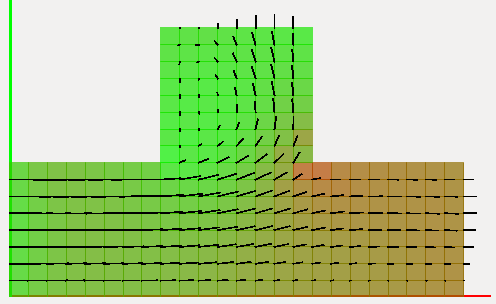
\includegraphics[width=0.7\linewidth]{stable.png}}
\end{figure}
\\
Тескер Констатин:
\begin{figure}[h!]
\center{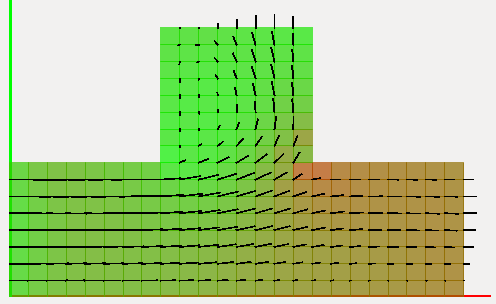
\includegraphics[width=0.7\linewidth]{stable.png}}
\end{figure}
\\
\\
Плотность газа характеризуется цветом ячейки. От зелёного к красному по возрастанию значения плотности. Черные палочки -- вектора скорости.

\newpage
\section{Сходимость и собственные функции}
Были проведены эксперименыты по скорости сходимости для изначального решения. Результаты приведены ниже.

Для матрицы были вычислено время установления стационарного решения и время восстановления его после возмущения. Были вычислены собственные значения
и их собственные вектора оператора линеаризации, а также проведены численные эксперименты, использующие полученные возмущения функций плотности и 
скорости. Ниже приведены результаты (возмущение считалось только для действительных собственных значений):
\begin{itemize}
 \item $-2.348801e-01$: время = 187
 \item $-1.784789e-01$: время = 315
 \item $-3.015234e-01 \pm 1.792826e-01$
 \item $-3.168194e-01 \pm 1.331842e-01$
 \item $-1.652393e-01 \pm 1.205335e-01$
\end{itemize}
Отсюда можно сделать вывод, что чем меньше собственное значение, тем быстрее оно сходится при малых возмущениях.
\section{Описание реализации}
Программа реализована на языке С, опираясь на исходный код выданной программы и используя пакет laspack.
Для реализации были созданы масивы инндексирующие связь плотности и скорости. Массивы назваются left bottom v - индекс скорости стоящей на пол узла ниже и пол узла левее плотности.
left h index -  индекс плотности на полл узла правее и пол узла выше узла скорости
left top h index -  индекс плотности на полл узла левее и пол узла выше узла скорости

nак же для облегчения работы с индексами были ввеедены два массива hv map и vh map jтвечающие за соответствие узлов скорости и плотности.

Для реализации заполнения сетки и начальных данныхбыли написаны функции set arrays for H, reset H index, setka for v.\\
Схема решения притерпела небольшие изменения. Вместо одного вычисления матрицы размерности $DIM_H + 2 \cdot DIM_V$ теперь используется две матрицы размерности $DIM_H$ для плотности  и размерности $2 * DIM_V$ для скорости. На каждом шаге по времени происходит сначала вычисление плотности по данным с предыдущего шага. Затем просиходит вычисление скорости по плотности с новго шага и значений сокрости с предыдущего шага. 

Для вычисления индексов для узла были добавлены функции fill for H и fill for v.
Для заполенения матриц использвуются функции cases H и case 0 V, case 1 8 V. Так как скорости на границах полагаются известными то разбирать случаи граничных узлов не имеет смысла, для них написан общий случай выставления диагонального элемента значение 1 и правой части с действительным значением скорости в этом узле.

Для запуска программы в режиме расчёта собственных значений необходимо задать переменную $USE\_EIGEN$ в файле "func.h" равной 1. Для запуска программы
в режиме линеаризации по известным собственным значениям необходимо задать эту переменную равной 0.

Для запуска программы в режиме расчёта собственных значений необходимо задать переменную $USE\_EIGEN$ в файле "func.h" равной 1. Для запуска программы
в режиме линеаризации по известным собственным значениям необходимо задать эту переменную равной 0.

Приведем графики скорости падения невязки при малых возмущениях, связянных с двумя действительными собственными значениями:

\newpage

\begin{figure}
 \centering	
 \begin{gnuplot}
  set terminal epslatex color size 12cm, 12cm
  set xzeroaxis lt -1
  set yzeroaxis lt -1
  set xrange [0:18]
  set style line 1 lt 1 lw 4 lc rgb '#ee0000' pt -1
  set style line 2 lt 1 lw 4 lc rgb '#008800' pt -1
  set grid xtics lc rgb '#555555' lw 1 lt 0
  set grid ytics lc rgb '#555555' lw 1 lt 0
  set key bottom right
  plot 'residual_4.log' using 1:2 with lines ls 1 ti '$eigen 4$', \
       'residual_7.log' using 1:2 with lines ls 2 ti '$eigen 7$'
  \end{gnuplot}
 \caption{Графики зависимости скорости падения невязки от собственного значения}
\end{figure} 

\section{Заключение}
В результате проведенных экспериментов было установлено, что схема даёт правдивые результаты и может быть использована для расчётов реальных моделей течения газов. 
\end{document}
